%&latex
%%----------------------------------------------------------------------
%% ieeepes_skel.tex
%%
%% Skeleton file for papers for the IEEE Power Engineering Society using
%% package ieeepes.
%%
%% Not copyrighted. Copy this file to a different name and fill in your
%% text.
%%
%% Volker Kuhlmann
%% c/o EEE Dept
%% University of Canterbury
%% Private Bag 4800
%% Christchurch, New Zealand
%% Email: KUHLMAV@ELEC.CANTERBURY.AC.NZ
%%
% 1.3  13Apr99  Updated for ieeepes 4.0.
% 1.2  16Nov95  Fixed discussion, closure. Added summary.
% 1.1  12Nov95  Finished first release.
% 1.02 09Nov95  Option PStimes.
% 1.0  07Nov95  Created.
%%----------------------------------------------------------------------
 
\documentclass[a4paper,twoside]{article}


\usepackage[%
               psphotos,      % uncomment those options you want
               photofit,%
        %       PStimes,%
        ]{ieeepes}



\title{Bus Tracking and Monitoring System Using RFID Technology}

\author{
        Mosab Wadea\\
        201021320
\and
        Omar Amin\\
        201073280
\and
        Ahmed Bajubair\\
        201152850
\and
        Mahdi Sahel\\
        201152070
}


\usepackage{graphicx}

\begin{document}

\maketitle


\begin{abstract}
Put the text of your abstract here.
\end{abstract}


%beginning sections
\section{Introduction}



\section{Problem}
The main transportation method in KFUPM is the bus system that is supervised and ran by the transportation department. The problem with the system depends on the knowledge of the student about the timing of the busses movements and when busses are located in any station. If a small delay or error happens in the system it will affect all the time schedule and the flow of the busses. This error is most likely to occur and can not be prevented. The problem with the students is that they will not be able to identify when a delay occurs and wither a bus is available or not.
%%%%%%%

\section{Solution}
The solution proposed in this project is to provide a monitoring system for both the student and the administrators. Where students can access a website to check for busses and their availability, as will as the administrators who can view the tracking results and evaluate the efficiency of the system.
%
\subsection{Requirements}
In order for the project to fulfill the needs it must sustain the following requirements:
\begin{itemize}
\item
Identify the busses and their assigned lines.
\item
Detect the busses and their movements.
\item
Detect busses on the run without the need to stop.
\item
Users can interact with the system and submit complaints.
\item
Administrators can access the system to evaluate the efficiency.
\item
Ability to accommodate multiple lines.
\end{itemize}
%
\subsection{Specifications}
In order to make these requirements feasible the project has to implement the following specifications:
\begin{itemize}
\item 
Attach RFID passive tag to each bus.
\item
Install RFID reader and antenna at each bus station.
\item
Develop web based application that connects to the readers and fitch data and displays them.
\end{itemize}
%%%%%

\section{Project Design}
The system is divided into two main parts, software and hardware. The software will contain the database, the communication with the reader as part of the back-end and the front-end which is the website of the service. The hardware consists mainly from the reader and the antennas as well as the tags attached to each bus. In \figref{blockdiagram} the block diagram shows how the software and hardware components work together.
\subsection{Block diagram}
In the block diagram seen in \figref{blockdiagram} there are three main components that interact with the system, the bus station which contains the readers and the antennas, the front-end that consists of the students interface and the administrators panel, the last component is the bus that is tagged with an RFID tag. All these components are linked together and processed in the server. The server contains the software that will be described in details in the next section.
\begin{figure}
\centering
\fbox{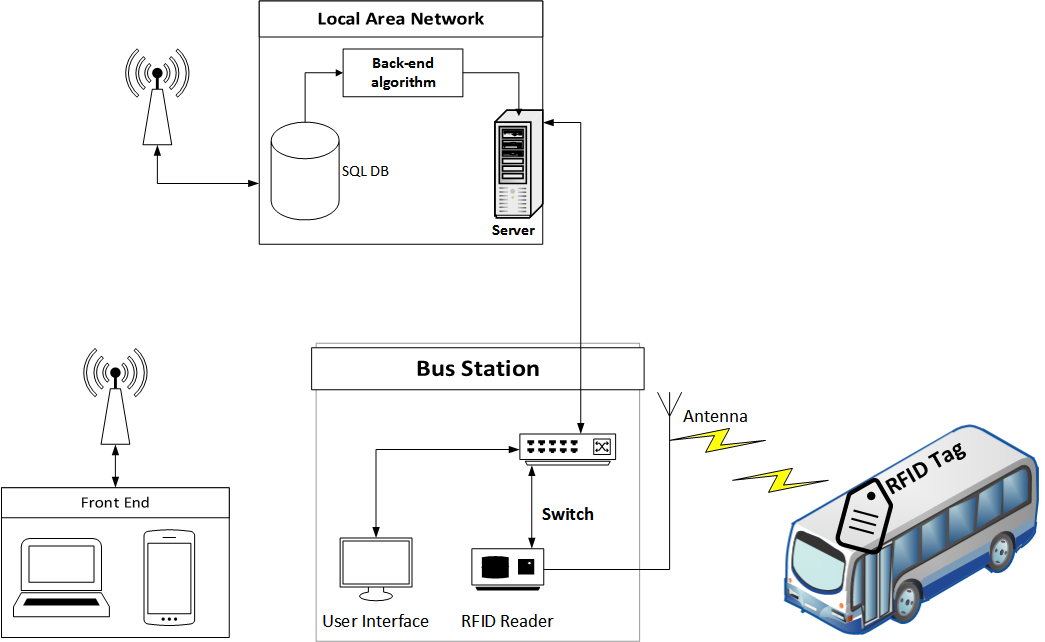
\includegraphics[scale=0.9]{blockdiagram/hardware.png}}
\caption{The block diagram of the system}
\label{blockdiagram}
\end{figure}
%
\subsection{Software architecture}
The software part is divided into three main parts as shown in \figref{blockdiagram} in the local area network tear, these three main parts are:
\begin{itemize}
\item
Back-end logic.
\item
The database.
\item
Web server.
\end{itemize}
The back-end contains a C\# code that the team developed. This code will communicate with the reader to check the busses available at each station and it will write these information in a database. The web server will communicate with the database to get the latest information and it will update the front-end interface without the need to refresh the page by the user. The database is constructed of the following tables:
\begin{itemize}
\item
Bus.
\item
Path.
\item
Line.
\item
Station.
\item
Log.
\end{itemize}
The entity model shown in \figref{entity} shows the database structure and the attributes for each entity.
\begin{figure}
\centering
\fbox{\includegraphics[scale=1.2]{blockdiagram/entity.png}}
\caption{The entity model of the database}
\label{entity}
\end{figure}


\section{Methodology}


\subsection{Hardware}
%add subsections here to place the test results

\subsection{Software}
%add subsections here to describe code



\section{Discussion}

\subsection{Challenges}

\subsection{limitations}



\section{Conclusion}






%this is the figure codes
% 
% \begin{figure}
% \centering
% \fbox{\includegraphics{c:/users/mosab/desktop/capture.png}}
% \caption{This is the caption for figure \#1.}
% \label{figure1}
% \end{figure}

%here is the table code
 
% \begin{table}
% \caption{This is the caption for table \#1. Make sure it goes
% \emph{before} the table!}
% \label{table1}
% \centering
% table matter
% \end{table}

%here is the refrencing codes

% Figure and table references: \figref{figure1}, \tabref{table1}. Use
% these at the beginning and within a sentence.




\end{document}

